\section{Лекция 3}
\subsection{\S XII.6. Стационарная теория возмущений для вырожденного спектра}

Пусть имеется  $s$-кратно вырожденный уровень энергии $E_n^{(0)}$. Пусть $\alpha$ --- индекс, нумерующий собственные векторы, соответствующие данному уровню, $\alpha = \overline{1, s}$. Тогда стационарное уравнение Шредингера записывается в виде

\[
\hat{H}_0\ket{E_{n\alpha}^{(0)}} = E_n^{(0)}\ket{E_{n\alpha}^{(0)}}
\]

С помощью ортогонализации всегда можно выбрать векторы так, что
$\braket{E_{n\alpha}^{(0)}}{E_{n\alpha'}^{(0)}} = \delta_{\alpha\alpha'}$.\\

Натянем на этот базис гильбертово пространство $\mathcal{H}_s^{(n)} \subset \mathcal{H}$.\\

Рассмотрим оператор возмущения:
$|V_{(n\alpha)(n\alpha')}| = |\braupket{E_{n\alpha}^{(0)}}{\hat{V}}{E_{n\alpha'}^{(0)}}| \ll$
\[
\ll \text{ из условия применимости стационарной теории } \ll |E_{n\alpha}^{(0)} - E_{n\alpha'}^{(0)}| = |E_{n}^{(0)} - E_{n}^{(0)}| =  0
\]
 $\Rightarrow$ противоречие $\Rightarrow$ построенная ранее теория не работает для вырожденного спектра.\\

В $\mathcal{H}_s^{(n)}$ имеется базис $\{\ket{E_{n\alpha}^{(0)}}\} \Rightarrow$ в этом базисе $\hat{H}_0$ представимо в виде:
\begin{figure}[H]
	\centering
	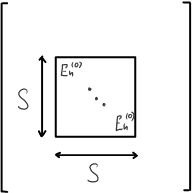
\includegraphics[width=0.2\linewidth]{images/l3_1.jpg}
\end{figure}

Введём в $\mathcal{H}_s^{(n)}$ другой базис $\ket{\psi_{n\beta}^{(0)}} = \displaystyle\sum\limits_{\alpha = 1}^s C_{\beta}^\alpha \ket{E_{n\alpha}^{(0)}}$ --- здесь все равно матрица $\hat{H}_0$ диагональна $\Rightarrow$ не важно, какой базис.\\

Выберем такой базис в $\mathcal{H}_s^{(n)}$, которые одновременно является набором собственных векторов $\hat{V}$, т.е. $\hat{V}\ket{\psi_{n\beta}^{(0)}} = V_{n\beta}\ket{\psi_{n\beta}^{(0)}}$. Такие векторы --- правильные векторы состояния нулевого приближения.\\

Подействуем $\hat{H}$: $\hat{H}\ket{\psi_{n\beta}^{(0)}} = (\hat{H}_0 + \hat{V})\ket{\psi_{n\beta}^{(0)}} = (E_n^{(0)} + V_{n\beta})\ket{\psi_{n\beta}^{(0)}}$ --- собственные векторы, соответствующие состоянию $E_{n\beta} = E_n^{(0)} + V_{n\beta}$ --- искомое расщепление.

\begin{figure}[H]
	\centering
	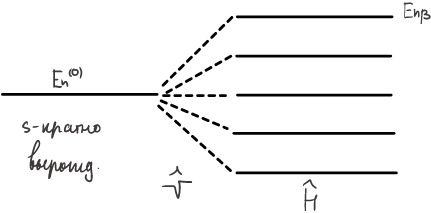
\includegraphics[width=0.75\linewidth]{images/l3_2.jpg}
\end{figure}

Как найти $\ket{\psi_{n\beta}^{(0)}}$?
\begin{enumerate}
	\item В имеющемся у нас базисе считаем $V_{(n\alpha)(n\alpha')} = \bra{E_{n\alpha}^{(0)}}\hat{V}\ket{E_{n\alpha'}^{(0)}}$.
	\item Решаем уравнение $\det(\hat{V} - \lambda\hat{1}) = 0$ и находим $\lambda_i$.
	\item $\hat{V}\ket{psi_{n\beta}^{(0)}} = \lambda_\beta\ket{\psi_{n\beta}^{(0)}}$ $\Rightarrow$ находим $\{\ket{\psi_{n\beta}^{(0)}}\}$.
\end{enumerate}

Данная теория может быть применена не только к $s$-кратно вырожденным уровням, но и к очень близким невырожденным.



\section{XIII. Стационарная теория рассеяния}

\subsection{\S XIII. Уравнение Липпмана~--- Швингера}

Пусть гамильтониан $\hat{H} = \hat{H}_0 + \hat{V}$.\\

Предположения, что:
\begin{enumerate}
	\item $\hat{H}$, $\hat{H}_0$ и $\hat{V}$ не зависят от времени.
	\item $\hat{H}_0$ имеет непрерывный спектр.
	\item Спектр $\hat{H}_0$ должен полностью принадлежать спектру $\hat{H}$.
	\item Рассмотрим $\hat{V}$ в координатном представлении $\Rightarrow$ ему отвечает функция $V(\vec{r})$. Тогда $\lim\limits_{|\vec{r}|=r\to\infty} V(\vec{r}) = 0$.
\end{enumerate}

\begin{example}
	$V(\vec{r}) = -g^2\,\dfrac{e^{-r/a}}{r}$, $a$ --- (эффективный) радиус действия потенциала.
	
	Внутри $a$ потенциал влияет на движение, иначе считаем $V(\vec{r}) = 0$.
\end{example}

\begin{example}
	$V(\vec{r}) \sim \dfrac{e^2}{r}$ --- имеет радиус действия $\infty$ (стремится к 0, но недостаточно быстро, чтобы этим пренебречь).
\end{example}

Рассмотрим задачу решения $(\hat{1}E - \hat{H})\ket{\psi} = 0$ в области непрерывного спектра (пусть для простоты только непрерывный спектр $\hat{H}$):

\begin{figure}[H]
	\centering
	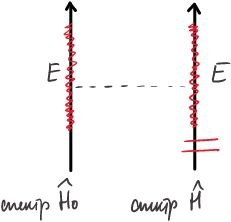
\includegraphics[width=0.3\linewidth]{images/l3_3.jpg}
\end{figure}

\[
(\hat{1}E - \hat{H}_0)\ket{\varphi^{(0)}} = 0, \qquad
\hat{G}_0^{(\pm)}(E) = (\hat{1}E - \hat{H}_0 \pm i\varepsilon)^{-1}
\]

\[
\Rightarrow (\hat{1}E - \hat{H}_0)\ket{\psi} = \hat{V}\ket{\psi}
\]

Если $\hat{V}$ достаточно мало $\Rightarrow \ket{\psi} = \ket{\varphi^{(0)}} + \ket{\delta\psi}$

\[
\hat{V}\ket{\psi} = (\hat{1}E - \hat{H}_0)(\ket{\varphi^{(0)}} + \ket{\delta\psi}) = (\hat{1}E - \hat{H}_0)\ket{\delta\psi}, \text{ домножим на слева на } \hat{G}_0
\]

\[
\Rightarrow \hat{G}_0(E)\hat{V}\ket{\psi} = \hat{G}_0(E)(\hat{1}E - \hat{H}_0)\ket{\delta\psi} = \ket{\delta\psi}
\qquad \Rightarrow \ket{\psi^{(\pm)}} = \ket{\varphi^{(0)}} + \hat{G}_0^{(\pm)}(E)\hat{V}\ket{\psi}
\]

\noindent --- собственно, это и есть искомое уравнение, но в большинстве книг \textbf{уравнение Липпмана~---Швингера:}
\[
\ket{\psi^{(\pm)}} = \ket{\varphi^{(0)}} + \frac{\hat{1}}{\hat{1}E - \hat{H}_0 \pm i\varepsilon}\,\hat{V}\ket{\psi^{(\pm)}}
\]

Для решения применяем метод итераций:
\begin{align*}
	1:&\quad \ket{\psi^{(1,\,\pm)}} = (\hat{1} + \hat{G}_0^{(\pm)}(E)\hat{V})\ket{\varphi^{(0)}}\\
	&\quad \text{Такое приближение называется \textbf{борновским}}\\[4pt]
	2:&\quad \text{подставляем в правую часть}\\
	&\;\vdots
\end{align*}

\[
\Rightarrow \ket{\psi^{(\pm)}} = \hat{1} + \sum_{s=1}^\infty \bigl(\hat{G}_0(E)\,\hat{V}\bigr)^s\ket{\varphi^{(0)}}
\]

\subsection{\S XIII.2. Упругое рассеяние и амплитуда рассеяния}

\begin{definition}
	Упругое рассеяние --- такое рассеяние, которое происходит без изменения сорта и числа частиц, и без изменения их внутренней энергии.
\end{definition}

\begin{example}
	\[
	p + Au \to p + Au, \qquad e^- + e^- \to e^- + e^-
	\]
\end{example}

\begin{definition}
	\textbf{Неупругое рассеяние} --- все то рассеяние, что не является упругим.
\end{definition}

\begin{example}
	\[
	e^- + e^- \longrightarrow e^- + e^- + \gamma
	\]
\end{example}

Рассмотрим задачу, изображенную на рисунке.

\begin{figure}[H]
	\centering
	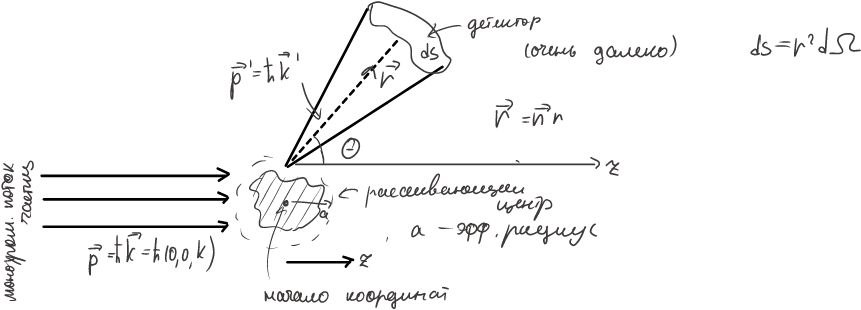
\includegraphics[width=1.0\linewidth]{images/l3_4.jpg}
\end{figure}
Пусть $\hat{H} = \hat{H}_0 + \hat{V}$, где $\hat{H}_0 = \dfrac{\hat{\vec{p}}^2}{2m}$ --- гамильтониан свободной частицы, $vec{p} = \hbar\vec{k}$, $E = \dfrac{\vec{p}^2}{2m} = \dfrac{\hbar^2}{2m}\vec{k}^2 \geq 0$, $r \gg a$.\\

\[
\hat{H}_0 = \dfrac{\hat{\vec{p}}^2}{2m} \Longrightarrow \ket{\varphi^{(0)}} = \ket{E = \dfrac{p^2}{2m}, \vec{p}}, \quad \hat{\vec{p}}\ket{\vec{p}} = \vec{p}\ket{\vec{p}}
\]
\[
\braket{\vec{r}}{\varphi^{(0)}} = \Psi_E(\vec{r}) = \dfrac{1}{\sqrt{V}} e^{\frac{i}{\hbar}\vec{p}\vec{r}} = \dfrac{1}{\sqrt{V}}e^{ikz}
\]
Для удобства считаем
\[
\braket{\vec{r}}{\psi^{(\pm)}} = \dfrac{1}{\sqrt{V}}\Psi^{(\pm)}(\vec{r})
\]

ТОгда уавнение Липпмана-Швингера в координатном представлении
\[
\Psi^{(\pm)}(\vec{r}) = e^{ikz} + \int d\vec{r'} G_0^{(\pm)}(E, \vec{r} - \vec{r'})V(\vec{r'})\Psi^{(\pm)}(\vec{r'})
\]

Каковы асимптотикаи $\Psi^{(\pm)}$ при $r \longrightarrow \infty$?
\[
|\vec{r} - \vec{r'}| = \sqrt{(\vec{r} - \vec{r'})^2} = \sqrt{\vec{r}^2 + \vec{r'}^2 - 2({\vec{r}\vec{r'})}} \approx \sqrt{\vec{r}^2 - 2({\vec{r}\vec{r'})}} \approx r\Big( 1 - \frac{(\vec{n}\vec{r'})}{r}\Big) = r - (\vec{n}\vec{r'})
\]

\[
\Longrightarrow G_0^{(\pm)}(E, \vec{r} - \vec{r'})\Big|_{r\longrightarrow\infty} = \dfrac{e^{\pm ikr}}{r}\Big(- \dfrac{m}{2\pi\hbar^2}\Big)e^{\mp i(\vec{k'}\vec{r'})}
\]

\[
\Longrightarrow Psi^{(\pm)}(\vec{r})\Big|_{r\longrightarrow\infty} = e^{ikz} + \dfrac{e^{\pm ikr}}{r}\int d\vec{r'}\Big(- \dfrac{m}{2\pi\hbar^2}\Big)e^{\mp i(\vec{k'}\vec{r'})}V(\vec{r'})\Psi^{(\pm)}(\vec{r'})
\]

Для решения из граничных условий выбираем
\[
Psi^{(+)}(\vec{r})\Big|_{r\longrightarrow\infty} = e^{ikz} + \dfrac{e^{ikr}}{r}f(\theta, \varphi)
\]

\begin{definition}
	\textbf{Амплитуда рассеяния} --- это
	\[
		f(\theta, \varphi) = - \dfrac{m}{2\pi\hbar^2}\int d\vec{r'} e^{-i(\vec{k'}\vec{r'})}V(\vec{r'})\Psi^{(+)}(\vec{r'})
	\]
\end{definition}

